\section{Kreiskollision}\index{Kreiskollision}
%%%%%%%%%%%%%%%%%%%%%%%%%%%%%%%%%%%%%%%%%%%%%%%%%%%%%%%%%%%%%%%%%%%%%

Während des Unterrichts wurde immer wieder einmal die Kollision zweier Bälle thematisiert. Ich habe deshalb hier eine einfache Simulation einer solchen Kollision programmiert. Ich gehe davon aus, dass die Techniken in \kapref{secGrundlagen} bekannt sind. In der Literatur finden Sie das Thema unter dem Schlagwort \gls{elakoll}.

%%%%%%%%%%%%%%%%%%%%%%%%%%%%%%%%%%%%%%%%%%%%%%%%%%%%%%%%%%%%%%%%%%%%%
\subsection{\reqref{reqBälle01}: Abprallen an den Rändern}

\br{Abprallen an den Rändern}{reqBälle01}
\begin{enumerate}
    \item Zwei Bälle mit unterschiedlicher zweidimensionales Geschwindigkeiten bewegen sich innerhalb einer Spielfläche.\label{reqBälle0101}
    \item Die Bälle prallen an den Ränder ab.\label{reqBälle0102}
    \item Das Spiel hat eine von der \emph{FPS} unabhängige Ablaufgeschwindigkeit.\label{reqBälle0103}
    \item Mit Hilfe der linken Maustaste wird ein neuer Ball platziert.\label{reqBälle0104}
    \item Mit Hilfe der rechten Maustaste wird ein Ball gelöscht.\label{reqBälle0105}
\end{enumerate}
\er

Die Präambel sollte keinerlei Fragen aufwerfen. Anhand der Variablen \texttt{DELTATIME} können Sie sehen, dass eine \texttt{FPS}-unabhängige Geschwindigkeit vorgesehen ist.  

\lstsource{SRC/01 Beispiele/02 Impuls/impuls00.py}{1}{17}{python}{Kreiskollision (\reqref{reqBälle01} -- Präambel
)}{srcImpuls00a}

Im Konstruktor der Klasse \texttt{Ball} wird das Image geladen und auf eine zufällig gewählte Größe skaliert. Geschwindigkeit und Position werden in zwei \texttt{pygame.math.Vector2}-Objekten\randnotiz{Vector2}\myindex{pyg}{\texttt{math}!\texttt{Vector2}} abgelegt. Dies verhindert, dass bei der Positionsberechnung später Nachkommastellen einfach abgeschnitten werden. 

\lstsource{SRC/01 Beispiele/02 Impuls/impuls00.py}{20}{32}{python}{Kreiskollision (\reqref{reqBälle01} -- Klasse \texttt{Ball}: Konstruktor)}{srcImpuls00b}

In \text{update()} wird zunächst die neue Position berechnet. Anschließend wird überprüft, ob der Ball die Spielfläche rechts oder links verlassen hat. Wenn ja, wird der Ball wieder an den Spielfeldrand positioniert, wobei jeweils $1~px$ Abstand gelassen wird; schließlich könnte ein schneller Ball innerhalb eines Frames ja schon die rechte oder linke Grenze weit -- also sichtbar -- überschritten haben. Danach wird das Vorzeichen der entsprechenden Geschwindigkeit vertauscht, wodurch der Effekt des Abprallens entsteht. Im Anschluss erfolgt die analoge Logik für die obere und untere Grenze der Spielfläche.

\lstsource{SRC/01 Beispiele/02 Impuls/impuls00.py}{34}{54}{python}{Kreiskollision (\reqref{reqBälle01} -- Klasse \texttt{Ball}: \texttt{update()})}{srcImpuls00c}

Die beiden Methoden \texttt{position2rect()} und \texttt{rect2position()} sorgen jeweils für den Datenaustausch mit dem \texttt{Rect}-Objekt des Sprite (siehe \srcref[vref]{srcImpuls00d}). In \texttt{select\-po\-si\-tion()} wird ein zufälliges Kreiszentrum ausgewählt. Um zu verhindern, dass die Kreise schon beim Start nicht vollständig innerhalb der Spielfläche liegen, wird ein um den Radius des Balls verkleinertes Rechteck erzeugt (\randnotiz{inflate()}\texttt{pygame.Rect.inflate()}-Objekten\myindex{pyg}{\texttt{Rect}!\texttt{inflate()}}). 



\lstsource{SRC/01 Beispiele/02 Impuls/impuls00.py}{56}{68}{python}{Kreiskollision (\reqref{reqBälle01} -- Klasse \texttt{Ball}: Hilfsfunktionen)}{srcImpuls00d}


In der Methode \texttt{selectimpulse()} wird eine Gesamtgeschwindigkeit und ein Winkel -- also ein \gls{impuls} -- geraten. Anschließend wird aus diesen beiden Werten die Geschwindigkeit in der Horizontalen und in der Vertikalen berechnet.

Wie kommen da jetzt auf einmal $\sin$ und $\cos$ ins Spiel? \randnotiz{$\sin()$, $\cos()$} Schauen wir uns dazu \abbref[vref]{picImpuls01} an. Wir haben hier den Ball. Dieser hat den Impuls~\textcolor{green!70!black}{$\vec{p}$}, der sich aus seiner Geschwindigkeit~\textcolor{green!70!black}{$v_{\vec{p}}$} und seiner Richtung~\textcolor{green!70!black}{$\alpha_{\vec{p}}$} zusammensetzt. Beide Informationen haben wir im Quelltext (\texttt{velocity}\textcolor{green!70!black}{$=v_{\vec{p}}$} bzw. \texttt{angle}\textcolor{green!70!black}{$=\alpha_{\vec{p}}$}) per Zufall ermittelt, sind also gegeben und daher \textcolor{green!70!black}{grün} markiert.


\begin{figure}[H]
	\begin{tikzpicture}\shorthandoff{"}
		\tikzset{>=latex} % for LaTeX arrow head
		\colorlet{myblue}{blue!65!black}
		\colorlet{myred}{red!65!black}
		\colorlet{mygreen}{green!70!black}
		\colorlet{vcol}{green!70!black}
		\colorlet{xcol}{blue!85!black}
		\tikzstyle{vector}=[->,very thick,line cap=round]
		\tikzstyle{direction} = [thick]
		\tikzstyle{xline}=[very thick]
		
		\def\maxx{9.0}
		\def\maxy{4.0}
		\def\r{0.6}
		\def\richtung{20.0}
		\def\geschwindigkeit{5.0}
		\def\Bx{1.0}
		\def\By{1.0}
		\def\Vx{\geschwindigkeit*cos(\richtung)}
		\def\Vy{\geschwindigkeit*sin(\richtung)}
		\def\Ix{{\Bx+\Vx}}
		\def\Iy{{\By+\Vy}}
		
		
		
		%Bildschirm Koordinatensystem
		\draw
		(0,0) node (o) {(0,0)}
		(0,\maxy) node (y) {y}
		(\maxx,0) node (x) {x}
		;
		\draw[->] (o) -- (x);
		\draw[->] (o) -- (y);
		
		%Ball
		\coordinate (B) at (\Bx, \By);
		%\draw[xline] (B) circle (\r); 
		\node (myfirstpic) at (B) {\includegraphics[scale=0.03]{blue2.png}};
		
		
		%Impuls
		\coordinate (Is) at (B);
		\coordinate (Ie) at (\Ix,\Iy);
		%\path (Is) +(\richtung:\geschwindigkeit) coordinate (Ie);
		\path (B) +(\richtung:0.5*\geschwindigkeit) coordinate (MyA);
		\path (B) +(0:0.5*\geschwindigkeit) coordinate (MyB);
		
		
		\draw[vector, mygreen] (Is) -- (Ie) node[above left=1, pos=0.9] {$v_{\vec{p}}$};
		\draw pic["\textcolor{mygreen}{$\alpha_{\vec{p}}$}", draw=mygreen, <->, angle eccentricity=0.8, angle radius=1.6cm]{angle=MyB--B--MyA};
		
		\draw[dashed, myred] (Is) -- (\Ix,\By) node[myred, below, pos=0.5] {$speed_x$};
		\draw[dashed, myred] (Ie) -- (\Ix,\By) node[myred, right, pos=0.5] {$speed_y$};
		
	\end{tikzpicture}
	\caption{Zerlegung des Impuls in horizontale und vertikale Vektoren}\label{picImpuls01}
\end{figure}

Gesucht werden die horizontale Geschwindigkeit \textcolor{red!65!black}{$speed_x$} und die vertikale \textcolor{red!65!black}{$speed_y$}. Diese werden daher \textcolor{red!65!black}{rot} markiert. Betrachtet man die gestichelten Linien -- die ja lediglich parallel verschobene $x$- und $y$-Achsen sind -- so erkennt man ein rechtwinkliges Dreieck (Hurra!). Und wie so oft in der Trigonometrie: Hat man erstmal das rechtwinklige Dreieck gefunden, so hat man gewonnen; dort gilt nämlich, das der Sinus eines Winkels der Quotient von Gegenkathete und Hypotenuse und der Cosinus der von Ankathete und Hypotenuse sind. Unser Winkel ist \textcolor{green!70!black}{$\alpha_{\vec{p}}$}, die Gegenkathete \textcolor{red!65!black}{$speed_y$} und die Ankathete \textcolor{red!65!black}{$speed_x$}. Daraus folgt:

\begin{eqnarray}
	\textcolor{green!70!black}{\sin(\alpha_{\vec{p}})} = \frac{\textcolor{red!65!black}{speed_x}}{\textcolor{green!70!black}{v_{\vec{p}}}} & \Longleftrightarrow &
	\textcolor{red!65!black}{speed_x} = \textcolor{green!70!black}{\sin(\alpha_{\vec{p}})} * \textcolor{green!70!black}{v_{\vec{p}}}\label{refSpeedx} \\
\nonumber \\
	\textcolor{green!70!black}{\cos(\alpha_{\vec{p}})} = \frac{\textcolor{red!65!black}{speed_y}}{\textcolor{green!70!black}{v_{\vec{p}}}} & \Longleftrightarrow &
	\textcolor{red!65!black}{speed_y} = \textcolor{green!70!black}{\cos(\alpha_{\vec{p}})} * \textcolor{green!70!black}{v_{\vec{p}}}\label{refSpeedy} 
\end{eqnarray}

Diese beiden Gleichungen \ref{refSpeedx} und \ref{refSpeedy} liefern mir jeweils Formeln zur Berechnung der beiden Geschwindigkeitsanteile. Verbleibt noch ein kleiner Stolperstein: Das Koordinatensystem der \abbref[vref]{picImpuls01} hat seinen 0-Punkt links unten. Je höher ein Punkt ist, desto \emph{größer} ist damit der y-Wert. In Pygame ist der Ursprung des Koordinatensystems aber links oben. Je höher der Punkt ist, desto \emph{kleiner} ist der y-Wert. Daher muss das Vorzeichen vor der Kosinusfunktion noch wechseln.

\lstsource{SRC/01 Beispiele/02 Impuls/impuls00.py}{70}{74}{python}{Kreiskollision (\reqref{reqBälle01} -- Klasse \texttt{Ball}: \texttt{selectimpulse()})}{srcImpuls00e}

Verbleibt noch die Klasse \texttt{Game} und der Programmaufruf. Mit \texttt{add\_ball()} und \texttt{remove\_ball()} werden \reqref{reqBälle0104} und \reqref{reqBälle0105} umgesetzt.

\lstsource{SRC/01 Beispiele/02 Impuls/impuls00.py}{77}{999}{python}{Kreiskollision (\reqref{reqBälle01} -- Klasse \texttt{Game} und Programmaufruf)}{srcImpuls00f}

Es erscheint ein Haufen Bälle, die von den Rändern abprallen (siehe \abbref[vref]{picKreiskollision01}) Die Bälle erkennen derzeit noch nicht, ob sie sich berühren, oder gar überlagern. 

\myebild{kreiskollision01.png}{1.0}{Umherfliegende Bälle}{picKreiskollision01}


%%%%%%%%%%%%%%%%%%%%%%%%%%%%%%%%%%%%%%%%%%%%%%%%%%%%%%%%%%%%%%%%%%%%%
\subsection{\reqref{reqBälle02}: Platzieren}

\br{Platzieren}{reqBälle02}
\begin{enumerate}
    \item Ein neuer Ball wird auf einer freien Fläche platziert.\label{reqBälle0201}
    \item Der Platz um den neuen Ball soll mindestens $5~px$ betragen.\label{reqBälle0202}
\end{enumerate}
\er

Für \reqref{reqBälle02}.\ref{reqBälle0201} muss lediglich die Methode \texttt{add\_ball()} erweitert werden. Nachdem wir einen Ball erzeugt haben, wird über \texttt{spritecollide()}\randnotiz{spritecollide()} \myindex{pag}{\texttt{sprite}!\texttt{spritecollide()}} ermittelt, ob der neue Ball mit einem der vorhandenen kollidiert. Dazu muss die Kollisionerkennung umgebogen werden. Per default macht \texttt{spritecollide()}eine Rechtecksprüfung, aber wir brauchen eine Kreiskollisionserkennung. Daher muss der Methode die entsprechende Kollisionerkennung als Parameter übergeben werden; hier ist es \texttt{collide\_circle()}\randnotiz{collide\_circle()}\myindex{pyg}{sprite!collide\_circle()}.

Gelingt dies nicht -- also kollidiert der neue Ball mit einem der älteren --, wird eine neue Position geraten und ein neuer Versuch gestartet. Dies passiert maximal 10 mal. Falls alle 10~Versuche erfolglos waren, wird der Ball einfach verworfen.

\lstsource{SRC/01 Beispiele/02 Impuls/impuls01.py}{124}{133}{python}{Kreiskollision (\reqref{reqBälle02}.\ref{reqBälle0201} -- \texttt{Game.add\_ball()})}{srcImpuls01a}

Aber was ist mit \reqref{reqBälle02}.\ref{reqBälle0202}? Hier verwenden wir einen kleinen Trick. Vor der Kollisionsprüfung erhöhen wir den Radius des neuen Balls um $5~px$ (\zeiref{srcImpuls01a01}) und danach reduzieren wir in wieder (\zeiref{srcImpuls01a02}).

\lstsource{SRC/01 Beispiele/02 Impuls/impuls01a.py}{124}{135}{python}{Kreiskollision (\reqref{reqBälle02}.\ref{reqBälle0202} -- \texttt{Game.add\_ball()})}{srcImpuls01aa}

%%%%%%%%%%%%%%%%%%%%%%%%%%%%%%%%%%%%%%%%%%%%%%%%%%%%%%%%%%%%%%%%%%%%%
\subsection{\reqref{reqBälle03}: Einfaches Abprallen zweier Bälle}

\br{Einfaches Abprallen}{reqBälle03}
Kollidieren zwei Bälle, sollen diese einfach ihre Richtung ändern.\label{reqBälle0301}
\er

Zuerst erweitern wir die Methode \texttt{Game.update()} um den Vergleich aller Bälle untereinander. Die beiden verschachtelten \forSchleife n halten dabei jeweils einen Ball fest und überprüfen diese mit allen anderen Bällen auf Kollision. Das Ergebnis ist verwirrend. Die Bälle prallen nicht ab, sondern durchwandern sich. Warum? Schauen wir uns dazu den linken Teil der \tabref[vref]{tabBallvergleich} an. Wenn Sie genau hinschauen, siehen Sie dass zwei Bälle während des Durchlaufs zweimal mit einenander auf Kollision überprüft werden; ein Beispiel\footnote{Damit der Text leichter zu lesen ist, wird der Ball mit dem Index~$i$ verkürzt als $Ball_i$ bezeichnet.}: $Ball_0~mit~Ball_2$ und $Ball_2~mit~Ball_0$. Wenn ich dann also zweimal das Vorzeichen wechsle, ist das Ergebnis so, als wenn ich das Vorzeichen der Geschwindigkeiten überhaupt nicht gewechselt hätte.

\lstsource{SRC/01 Beispiele/02 Impuls/impuls02.py}{116}{120}{python}{Kreiskollision (\reqref{reqBälle03}.\ref{reqBälle0301} -- \texttt{Game.update()}, nicht korrigiert)}{srcImpuls02a}

Lösung: Wenn wir $Ball_0$ festhalten, ist es nur sinnvoll diese mit allen Bällen $Ball_j$ zu vergleichen, für welche $j > 0$ ist. Machen Sie sich schnell klar, das in der inneren \forSchleife\ bei $j=0$ der $Ball_0$ mit sich selbst auf Kollision überprüft werden würde. Beim zweiten Durchlauf der äußeren \forSchleife\ ist $i = 1$. Diesen Ball nun wieder mit dem $Ball_0$ zu überprüfen, ist überflüssig, da diese Überprüfung schon beim ersten Schleifendurchlauf passiert ist. Wir brauchen daher die innere \forSchleife\ nicht bei~0 starten lassen, sondern mit dem nächst höheren Index, also $j = 2$. Verallgemeinert man diesen Gedanken, so braucht man $Ball_i$ immer nur mit $Ball_j$ bei $j > i$ zu überprüfen. Daher startet die innere \forSchleife\ auch nicht mit \texttt{0}, sondern \texttt{i+1}. Aus dem gleichen Grund endet die äußere \forSchleife\ auch nicht beim letzten, sondern beim vorletzten Index.

\lstsource{SRC/01 Beispiele/02 Impuls/impuls02a.py}{116}{120}{python}{Kreiskollision (\reqref{reqBälle03}.\ref{reqBälle0301} -- \texttt{Game.update()}, korrigiert)}{srcImpuls02a}

Da dieser Gedanke im Unterricht gelegentlich zu Verwirrung führt, habe ich die Bälle, die verglichen werden, in \tabref[vref]{tabBallvergleich} dargestellt. Auf der linken Seite sind die nicht korrigierten Schleifendurchläufe angegeben. Die definitiv unsinnigen sind \textcolor{red!65}{dunkelrot} und die doppelten \textcolor{red!30}{hellrot} eingefärbt. Es fällt auf -- hoffentlich --, dass nur die Vergleiche übrig bleiben, die auf der rechten Seite verzeichnet sind.
\small
\begin{longtable}{llp{3cm}|llp{3cm}}
	% Definition des Tabellenkopfes auf der ersten Seite
	\caption{Übersicht, welche Bälle überprüft werden (n=4)}\label{tabBallvergleich} \\
    \multicolumn{3}{c}{nicht korrigierte Version} & \multicolumn{3}{c}{korrigierte Version} \\ \hline
    \multicolumn{2}{c}{Schleifen} &  & \multicolumn{2}{c}{Schleifen} & \\ %\cline{1-2} \cline{4-5}
    äußere & innere & & äußere & innere & \\ %\cline{1-2} \cline{4-5}
	$i$    & $j$ & kollidiert? & $i$    & $j$ & kollidiert? \\\hline\hline
	\endfirsthead % Erster Kopf zu Ende
	% Definition des Tabellenkopfes auf den folgenden Seiten
	\caption{Übersicht, welche Bälle überprüft werden (n=4) (Fortsetzung)}\\
    \multicolumn{3}{c}{nicht korrigierte Version} & \multicolumn{3}{c}{korrigierte Version} \\ \hline
    \multicolumn{2}{c}{Schleifen} &  & \multicolumn{2}{c}{Schleifen} & \\ %\cline{1-2} \cline{4-5}
    äußere & innere & & äußere & innere & \\ %\cline{1-2} \cline{4-5}
	$i$    & $j$ & kollidiert? & $i$    & $j$ & kollidiert? \\\hline\hline
	\endhead % Zweiter Kopf ist zu Ende
	% Ab hier kommt der Inhalt der Tabelle
    0  &  0 & \cellcolor{red!65}$Ball_0$ mit $Ball_0$ & 0  &  1 & $Ball_0$ mit $Ball_1$\\ \hline
    0  &  1 &                   $Ball_0$ mit $Ball_1$ & 0  &  2 & $Ball_0$ mit $Ball_2$\\ \hline
    0  &  2 &                   $Ball_0$ mit $Ball_2$ & 0  &  3 & $Ball_0$ mit $Ball_3$\\ \hline
    0  &  3 &                   $Ball_0$ mit $Ball_3$ & 1  &  2 & $Ball_1$ mit $Ball_2$\\ \hline
    1  &  0 & \cellcolor{red!30}$Ball_1$ mit $Ball_0$ & 1  &  3 & $Ball_1$ mit $Ball_3$\\ \hline
    1  &  1 & \cellcolor{red!65}$Ball_1$ mit $Ball_1$ & 2  &  3 & $Ball_2$ mit $Ball_3$\\ \hline
    1  &  2 &                   $Ball_1$ mit $Ball_2$ &    &    &                       \\ \cline{1-3}
    1  &  3 &                   $Ball_1$ mit $Ball_3$ &    &    &                       \\ \cline{1-3}
    2  &  0 & \cellcolor{red!30}$Ball_2$ mit $Ball_0$ &    &    &                       \\ \cline{1-3}
    2  &  1 & \cellcolor{red!30}$Ball_2$ mit $Ball_1$ &    &    &                       \\ \cline{1-3}
    2  &  2 & \cellcolor{red!65}$Ball_2$ mit $Ball_2$ &    &    &                       \\ \cline{1-3}
    2  &  3 &                   $Ball_2$ mit $Ball_3$ &    &    &                       \\ \cline{1-3}
    3  &  0 & \cellcolor{red!30}$Ball_3$ mit $Ball_0$ &    &    &                       \\ \cline{1-3}
    3  &  1 & \cellcolor{red!30}$Ball_3$ mit $Ball_1$ &    &    &                       \\ \cline{1-3}
    3  &  2 & \cellcolor{red!30}$Ball_3$ mit $Ball_2$ &    &    &                       \\ \cline{1-3}
    3  &  3 & \cellcolor{red!65}$Ball_3$ mit $Ball_3$ &    &    &                       \\ \cline{1-3}
\end{longtable} 
\normalsize

Die Methode \texttt{ball\_collision()} checkt nun, ob die beiden Kreise kollidieren und dreht anschließend die Geschwindigkeitsvektoren um.

\lstsource{SRC/01 Beispiele/02 Impuls/impuls02.py}{144}{147}{python}{Kreiskollision (\reqref{reqBälle03}.\ref{reqBälle0301} -- \texttt{Game.ball\_collision()})}{srcImpuls02b}

Wenn Sie sich das Ergebnis allerdings anschauen, ist es eher enttäuschend. Die Bälle verhalten sich nicht annähernd so, wie man es von abprallenden Bällen zu sehen gewohnt ist. Grund ist, dass wir in \srcref[vref]{srcImpuls02b} einfach nur die Vorzeichen der beiden Geschwindigkeiten wechseln. Dies entspricht einer Spiegelung (Abprallen) an der $x$- bzw. $y$-Achse, weshalb das auch gut beim Abprallen an den Wänden funktionniert (siehe \srcref[vref]{srcImpuls00c}). Wir müssen also besser werden.


%%%%%%%%%%%%%%%%%%%%%%%%%%%%%%%%%%%%%%%%%%%%%%%%%%%%%%%%%%%%%%%%%%%%%
\subsection{\reqref{reqBälle04}: Elastisches Abprallen zweier Bälle}

\br{Elastisches Abprallen}{reqBälle04}
\begin{itemize}
    \item Kollidieren zwei Bälle, sollen diese unter Beachtung des Impuls ihre Richtungen ändern.\label{reqBälle0401}
    \item Die Masse der beiden Bälle soll ebenfalls berücksichtigt werden.\label{reqBälle0402}
\end{itemize}
\er

Wenn zwei Bälle aufeinander treffen, ist das aus der Perspektive eines Balles so, als ob er gegen eine Wand stößt. Damit der Ball nun im richtigen Winkel abprallen kann, müssen wir daher eine Wand am Berührungspunkt denken, die genau so ausgerichtet ist, dass sie zu den Bewegungen der beiden Bälle passt -- also nicht einfach senkrecht oder waagerecht. Dies wäre eine Wand, die beide Bälle nur in einem einzigen Punkt berührt, nämlich dem Punkt, wo beide aufeinander treffen. Und wie heißt eine Gerade, die etwas nur in einem Punkt berührt? Richtig \gls{tangente}\randnotiz{Tangente}\index{Tangente}. In \abbref[vref]{picImpuls02} ist dies die gestrichelte grüne Gerade~$t$. Machen Sie sich bitte klar, dass jede andere Ausrichtung dieser Gerade, die Kreisgrenzen nicht nur berühren, sondern auch schneiden würden.

Wie kann ich nun die Tangente berechnen? Hilfreich ist dabei die Beobachtung, dass die Tangente~$t$ senkrecht zur Verbindungsstrecke der beiden Ballmittelpunkte ist. In \abbref[vref]{picImpuls02} ist dies die gestrichelte grüne Linie~$n$. Dieser Vektor~$n$ () läßt sich einfach berechnen:

\begin{eqnarray}
	n  & = & B_1 - B_2 \nonumber \\
    {x_n \choose y_n} & = & {x_1 \choose y_1} - {x_2 \choose y_2} \label{eqNormvektor}
\end{eqnarray}

Den Vektor~$n$ zu berechenen, der senkrecht auf einer Linie steht (\gls{orthogonale}, \gls{normale}\randnotiz{Normale}\index{Normale})), ist wiederum recht einfach. Zwei Vektoren sind orthogonal zu einander, wenn ihr Vektorprodukt gleich~0 ist:
\begin{eqnarray}
	<n, t>                & = & 0 \Longleftrightarrow \nonumber \\
    n_x * t_x + n_y * t_y & = & 0 \Longleftrightarrow \label{eqOrthoAllg}
\end{eqnarray}

Eine Lösung für Gleichung~\ref{eqOrthoAllg} ist:
\begin{eqnarray}
	{t_x \choose t_y} & = & {-n_y \choose n_x}\Longrightarrow \label{eqOrthoSpez} \\
\end{eqnarray}

Bestätigen wir uns das schnell, indem wir \ref{eqOrthoSpez} in \ref{eqOrthoAllg} einsetzen:

\begin{eqnarray}
    n_x * (-n_y) + n_y * (n_x) & = & 0 \Longleftrightarrow \nonumber \\
    n_x * (-n_y + n_y) & = & 0 \Longleftrightarrow \nonumber\\
    n_x * (0) & = & 0 \nonumber
\end{eqnarray}

So, nun haben wir endlich die Tangente. Wie spiegeln wir nun die Impulsvektoren an der Tangente? Ähnlich wie beim Abprallen an den Außenwänden, nur das die Wand hier die Tangente ist. Beim Abprallen an der linken oder rechten Wand wird die horizontale Geschwindigkeit verändert, die vertikale bleibt gleich. Wir müssen also den Impulsvektor in seine zwei Teilvektoren aufspalten, aber eben nicht den horizontalen und den vertikalen, sondern den tangentialen Anteil und den normalen Anteil.

Dies passiert mit ein wenig Mathe recht schnell. Nehmen wir beispielsweise den Impuls~$\vec{p}_1$. Diesen in zwei Komponenten zu zerlegen, bedeutet, dass er als Linearkombination der beiden Vektoren~$t_1$ und ~$n_1$ geschrieben werden kann:

\begin{eqnarray}
    \vec{p}_1 & = & a * t_1 + b * n_1 \Longleftrightarrow \nonumber \\
    {p_x \choose p_y} & = & a * {t_x \choose t_y} + b * {n_x \choose n_y} \Longleftrightarrow \nonumber\\
    p_x & = & a * t_x + b * n_x \wedge \label{eqGlsZerlegung01}\\
    p_y & = & a * t_y + b * n_y  \nonumber
\end{eqnarray}

Das Gleichungssystem~\ref{eqGlsZerlegung01} hat zwei Gleichungen und zwei Unkekannte, den die Normale~$n$ also auch die Tangente~$t$ haben wir oben ermittelt. Wir können diese beiden Unbekannten also mit den üblichen Verfahren bestimmen und erhalten:

\begin{eqnarray}
    a & = & (p_x * n_y - p_y * n_x) / (t_x * n_y - t_y * n_x) \wedge \label{eqGlsZerlegung02} \\
    b & = & (p_y * t_x - t_y * p_x) / (t_x * n_y - t_y * n_x) \label{eqGlsZerlegung03}
\end{eqnarray}

Wir haben also jetzt für beide Impulsvektoren Formeln, die uns die jweils beiden Geschwindigkeitsvektoren liefern. Und jetzt wird wie beim Abprallen an der Wand der entsprechende Geschwindigkeitsvektor negiert und anschließend der neue Impulsvektor wieder zusammengebastelt. 

Welcher Geschwindigkeitsvektor wird nun negiert? Wenn wir uns die \abbref[vref]{picImpuls02} anschauen, dann haben wir eine Intuition, wohin die abgeprallten Bälle fliegen. Sie fliegen weiter nach unten, aber entfernen sich wieder voneinander. In unserer Mathe-Sprache übersetzt, würde man sagen, die Normalenanteile~$n_1$ und~$n_2$ bleiben unverändert und das Vorzeichen der Tangentenanteile~$t_1$ und~$t_2$ verändern sich.

\begin{figure}[H]
	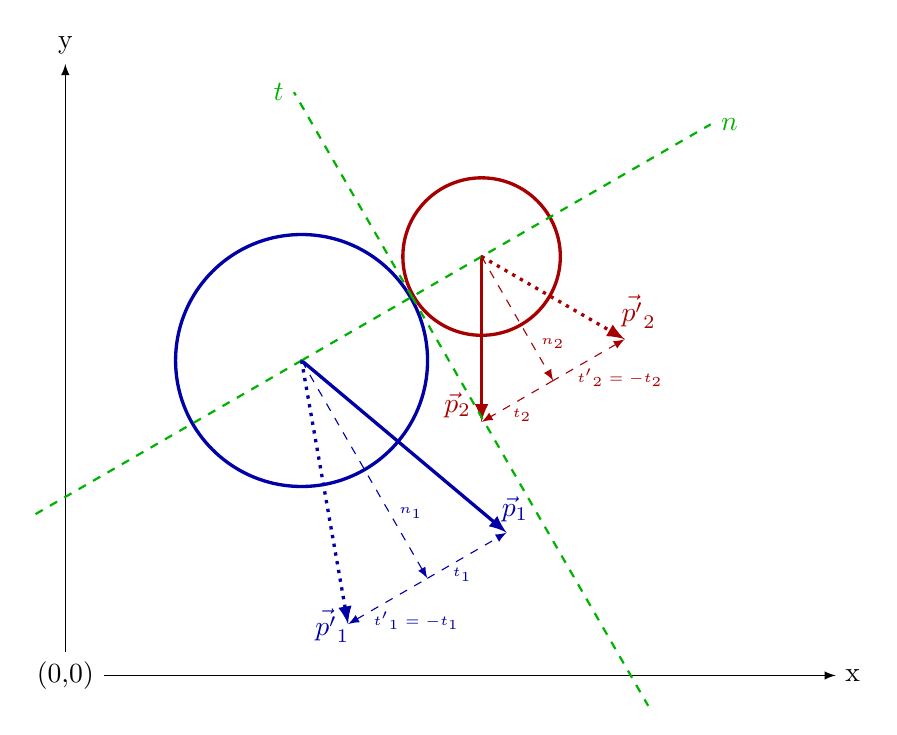
\begin{tikzpicture}\shorthandoff{"}
		\tikzset{>=latex} % for LaTeX arrow head
		\colorlet{myblue}{blue!65!black}
		\colorlet{myred}{red!65!black}
		\colorlet{mygreen}{green!70!black}
		\colorlet{vcol}{green!70!black}
		\colorlet{xcol}{blue!85!black}
		\tikzstyle{vector}=[->,very thick,line cap=round]
		\tikzstyle{direction} = [thick]
		\tikzstyle{xline}=[very thick]
		
        \def\ABNWinkel{30}
        \def\ABTWinkel{\ABNWinkel+90}
	
		%Bildschirm Koordinatensystem
		\def\maxx{10.0}
		\def\maxy{8.0}
		\draw
    		(0,0) node (o) {(0,0)}
	       	(0,\maxy) node (y) {y}
	   	   (\maxx,0) node (x) {x}
		;
		\draw[->] (o) -- (x);
		\draw[->] (o) -- (y);
		
		%Ball A
		\def\Aradius{1.6}
		\def\Arichtung{320.0}
		\def\Ageschwindigkeit{3.4}
		\def\Ax{3.0}
		\def\Ay{4}
		\coordinate (A) at (\Ax, \Ay);
		\draw[very thick, myblue] (A) circle (\Aradius); 
        % Impuls A
		\path (A) +(\Arichtung:\Ageschwindigkeit) coordinate (Aimpuls);
        \draw[vector, myblue] (A) -- (Aimpuls) node[above, xshift=3, pos=1.0] {$\vec{p}_1$};

		%Ball B
		\def\Bradius{1.0}
		\def\Brichtung{270.0}
		\def\Bgeschwindigkeit{2.1}
		\path (A) +(\ABNWinkel:{\Aradius + \Bradius + 0.04}) coordinate (B);
		\draw[very thick, myred] (B) circle (\Bradius); 
        % Impuls B
		\path (B) +(\Brichtung:\Bgeschwindigkeit) coordinate (Bimpuls);
        \draw[vector, myred] (B) -- (Bimpuls) node[left, pos=0.9] {$\vec{p}_2$};

        %Berührungspunkt
		\path (A) +(\ABNWinkel:{\Aradius + 0.02}) coordinate (K);
        
        %Tangente
        \draw [dashed, mygreen, thick] (K) -- +({\ABTWinkel}:3.0) node[left] {$t$};
        \draw [dashed, mygreen, thick] (K) -- +({\ABTWinkel+180}:6);

        %Normale
        \draw [dashed, mygreen, thick] (A) -- +(\ABNWinkel:6) node[right] {$n$};
        \draw [dashed, mygreen, thick] (A) -- +({\ABNWinkel+180}:4);

        %Split von a
        \def\AWN{(\Arichtung - (\ABTWinkel + 180)))} 
        \path (A) +(\ABTWinkel+180:{cos(\AWN)) * \Ageschwindigkeit}) coordinate (NA); 
        \draw [dashed, myblue, ->](A) -- (NA) node[right,pos=0.7] {\tiny $n_1$};
        \draw [dashed, myblue, ->](NA) -- (Aimpuls) node[right, pos=0.2, yshift=-2] {\tiny $t_1$};

        %Split von b
        \def\BWN{(\Brichtung - (\ABTWinkel + 180)))} 
        \path (B) +(\ABTWinkel+180:{cos(\BWN)) * \Bgeschwindigkeit}) coordinate (NB);
        \draw [dashed, myred, ->](B) -- (NB) node[right,pos=0.7] {\tiny $n_2$};
        \draw [dashed, myred, ->](NB) -- (Bimpuls) node[right, pos=0.7, yshift=-2] {\tiny $t_2$};

        %Spiegel von Impuls A
		\path (A) +({\Arichtung-2*\AWN}:\Ageschwindigkeit) coordinate (AAimpuls);
        \draw[dotted, very thick, myblue, ->] (A) -- (AAimpuls) node[below, xshift=-4, pos=0.9] {$\vec{p'}_1$};
        \draw [dashed, myblue, <-](AAimpuls) -- (NA) node[right, pos=0.2, yshift=-2] {\tiny ${t'}_1=-t_1$};

        %Spiegel von Impuls B
		\path (B) +({\Brichtung-2*\BWN}:\Bgeschwindigkeit) coordinate (BBimpuls);
        \draw[dotted, very thick, ->, myred] (B) -- (BBimpuls) node[above, pos=1.0, xshift=5] {$\vec{p'}_{2}$};
        \draw [dashed, myred, <-](BBimpuls) -- (NB) node[right, pos=0.8, yshift=-2] {\tiny ${t'}_2=-t_2$};


		
	\end{tikzpicture}
	\caption{Kollision zweier Bälle}\label{picImpuls02}
\end{figure}



\begin{figure}[H]
	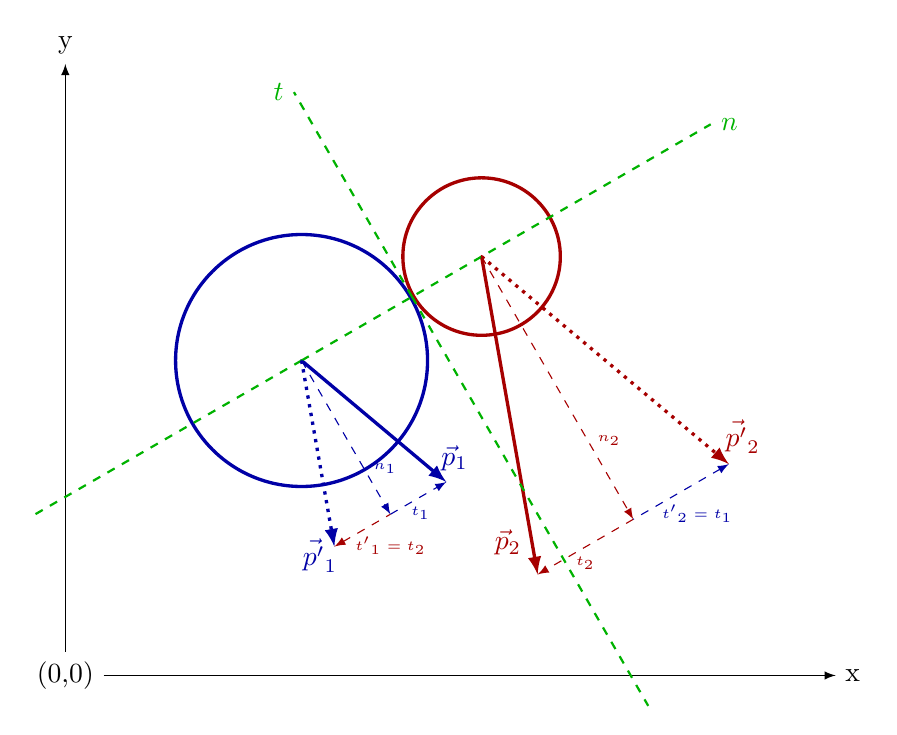
\begin{tikzpicture}\shorthandoff{"}
		\tikzset{>=latex} % for LaTeX arrow head
		\colorlet{myblue}{blue!65!black}
		\colorlet{myred}{red!65!black}
		\colorlet{mygreen}{green!70!black}
		\colorlet{vcol}{green!70!black}
		\colorlet{xcol}{blue!85!black}
		\tikzstyle{vector}=[->,very thick,line cap=round]
		\tikzstyle{direction} = [thick]
		\tikzstyle{xline}=[very thick]
		
		\def\ABNWinkel{30}
		\def\ABTWinkel{\ABNWinkel+90}
		
		%Bildschirm Koordinatensystem
		\def\maxx{10.0}
		\def\maxy{8.0}
		\draw
		(0,0) node (o) {(0,0)}
		(0,\maxy) node (y) {y}
		(\maxx,0) node (x) {x}
		;
		\draw[->] (o) -- (x);
		\draw[->] (o) -- (y);
		
		%Ball A
		\def\Aradius{1.6}
		\def\Arichtung{320.0}
		\def\Ageschwindigkeit{2.4}
		\def\Ax{3.0}
		\def\Ay{4}
		\coordinate (A) at (\Ax, \Ay);
		\draw[very thick, myblue] (A) circle (\Aradius); 
		% Impuls A
		\path (A) +(\Arichtung:\Ageschwindigkeit) coordinate (Aimpuls);
		\draw[vector, myblue] (A) -- (Aimpuls) node[above, xshift=3, pos=1.0] {$\vec{p}_1$};
		
		%Ball B
		\def\Bradius{1.0}
		\def\Brichtung{280.0}
		\def\Bgeschwindigkeit{4.1}
		\path (A) +(\ABNWinkel:{\Aradius + \Bradius + 0.04}) coordinate (B);
		\draw[very thick, myred] (B) circle (\Bradius); 
		% Impuls B
		\path (B) +(\Brichtung:\Bgeschwindigkeit) coordinate (Bimpuls);
		\draw[vector, myred] (B) -- (Bimpuls) node[left, pos=0.9] {$\vec{p}_2$};
		
		%Berührungspunkt
		\path (A) +(\ABNWinkel:{\Aradius + 0.02}) coordinate (K);
		
		%Tangente
		\draw [dashed, mygreen, thick] (K) -- +({\ABTWinkel}:3.0) node[left] {$t$};
		\draw [dashed, mygreen, thick] (K) -- +({\ABTWinkel+180}:6);
		
		%Normale
		\draw [dashed, mygreen, thick] (A) -- +(\ABNWinkel:6) node[right] {$n$};
		\draw [dashed, mygreen, thick] (A) -- +({\ABNWinkel+180}:4);
		
		%Split von a
		\def\AWN{(\Arichtung - (\ABTWinkel + 180)))} 
		\path (A) +(\ABTWinkel+180:{cos(\AWN)) * \Ageschwindigkeit}) coordinate (NA); 
		\draw [dashed, myblue, ->](A) -- (NA) node[right,pos=0.7] {\tiny $n_1$};
		\draw [dashed, myblue, ->](NA) -- (Aimpuls) node[right, pos=0.2, yshift=-2] {\tiny $t_1$};
		
		%Split von b
		\def\BWN{(\Brichtung - (\ABTWinkel + 180)))} 
		\path (B) +(\ABTWinkel+180:{cos(\BWN)) * \Bgeschwindigkeit}) coordinate (NB);
		\draw [dashed, myred, ->](B) -- (NB) node[right,pos=0.7] {\tiny $n_2$};
		\draw [dashed, myred, ->](NB) -- (Bimpuls) node[right, pos=0.7, yshift=-2] {\tiny $t_2$};
		
		%Spiegel von Impuls A
		\path (A) +({\Arichtung-2*\AWN}:\Ageschwindigkeit) coordinate (AAimpuls);
		\draw[dotted, very thick, myblue, ->] (A) -- (AAimpuls) node[below, xshift=-4, pos=0.9] {$\vec{p'}_1$};
		\draw [dashed, myred, <-](AAimpuls) -- (NA) node[right, pos=0.2, yshift=-2] {\tiny ${t'}_1=t_2$};
		
		%Spiegel von Impuls B
		\path (B) +({\Brichtung-2*\BWN}:\Bgeschwindigkeit) coordinate (BBimpuls);
		\draw[dotted, very thick, ->, myred] (B) -- (BBimpuls) node[above, pos=1.0, xshift=5] {$\vec{p'}_{2}$};
		\draw [dashed, myblue, <-](BBimpuls) -- (NB) node[right, pos=0.8, yshift=-2] {\tiny ${t'}_2=t_1$};
		
		
		
	\end{tikzpicture}
	\caption{Elastische Kollision zweier Bälle}\label{picImpuls03}
\end{figure}


\subsection*{Quellen}

Grundlagen und Programmierbeispiele finden Sie hier:
 
\begin{itemize}
	\item Wikipediaeintrag zur \href{https://en.wikipedia.org/wiki/Elastic_collision}{Elastischen Kollision}
    \item Ein fehlerhafter, aber lehrreicher Ansatz der Hochschule Augsburg: \url{https://glossar.hs-augsburg.de/Kollision_zweier_Kugeln_(2D)}
    \item Ein Beispiel für zwei Kugeln mit gleicher Masse: \url{https://peterloos.de/legacy/index.php/m-wpf/m-wpf-animations/70-a-wpf-elasticimpact}
    \item Meine Quelle zu ähnlichen Dreiecken: \url{https://de.bettermarks.com/mathe/aehnlichkeit-von-dreiecken/}
\end{itemize}

